% !TEX program = pdflatex
\documentclass[aspectratio=169,11pt]{beamer}

% ---------- Look & Feel ----------
\usepackage[T1]{fontenc}
\usepackage[utf8]{inputenc}
\usepackage{lmodern}      % good default sans + math with pdfLaTeX
\renewcommand{\familydefault}{\sfdefault}
\usepackage{microtype}
\usepackage{graphicx}
\usepackage{xcolor}
\usepackage{hyperref}
\usepackage{tikz}
\usetikzlibrary{arrows.meta,positioning,shapes.geometric}
\usepackage{tabularx}

% Color palette (C++-flavored, high contrast but soft)
\definecolor{CXXBlue}{RGB}{0,89,156}   % primary
\definecolor{Accent}{RGB}{230,93,36}   % highlight
\definecolor{Ink}{RGB}{33,36,41}       % text
\definecolor{Slate}{RGB}{99,110,123}   % secondary text
\definecolor{Light}{RGB}{245,247,250}  % gentle panel bg
\definecolor{Line}{RGB}{223,227,232}   % hairline

% Global beamer colors
\setbeamercolor{normal text}{fg=Ink,bg=white}
\setbeamercolor{structure}{fg=CXXBlue}
\setbeamercolor{frametitle}{fg=Ink,bg=Light}
\setbeamercolor{title}{fg=Ink}
\setbeamercolor{subtitle}{fg=Slate}
\setbeamercolor{block title}{fg=Ink,bg=Light}
\setbeamercolor{block body}{fg=Ink,bg=white}
\setbeamercolor{alerted text}{fg=Accent}
\setbeamercolor{itemize item}{fg=CXXBlue}
\setbeamercolor{itemize subitem}{fg=Slate}
\setbeamercolor{footline}{fg=Slate,bg=white}

% Fonts & sizes
\setbeamerfont{title}{series=\bfseries,size=\LARGE}
\setbeamerfont{frametitle}{series=\bfseries,size=\Large}
\setbeamerfont{subtitle}{size=\large}
\setbeamerfont{block title}{series=\bfseries}
\setbeamerfont{footline}{size=\scriptsize}

% Clean up navigation
\setbeamertemplate{navigation symbols}{}

% Better bullets
\setbeamertemplate{itemize item}{\raisebox{0.2ex}{\small$\blacktriangleright$}}
\setbeamertemplate{itemize subitem}{\raisebox{0.2ex}{\tiny$\bullet$}}

% Frametitle with slim accent rule
\setbeamertemplate{frametitle}{
  \nointerlineskip
  \begin{beamercolorbox}[wd=\paperwidth,ht=2.2em,dp=0.6em,leftskip=1.2em,rightskip=1.2em]{frametitle}
    \usebeamerfont{frametitle}\insertframetitle
  \end{beamercolorbox}
  \begin{beamercolorbox}[wd=\paperwidth,ht=0.3ex]{structure}\end{beamercolorbox}
}

% Minimal footline: title • frame number
\setbeamertemplate{footline}{
  \leavevmode%
  \hbox{\begin{beamercolorbox}[wd=\paperwidth,ht=3ex,dp=1.2ex,leftskip=1.2em,rightskip=1.2em]{footline}
    \insertshorttitle\hfill \insertframenumber/\inserttotalframenumber
  \end{beamercolorbox}}
}

% Section dividers
\newcommand{\sectionframe}[1]{%
  \begin{frame}[plain]
    \vfill
    \centering
    {\usebeamerfont{title}\color{CXXBlue}#1\par}
    \vspace{0.5em}
    \begin{beamercolorbox}[wd=0.35\paperwidth,ht=0.35ex,center]{structure}\end{beamercolorbox}
    \vfill
  \end{frame}
}
\AtBeginSection{\sectionframe{\insertsectionhead}}

% Hyperref coloring
\hypersetup{
  colorlinks=true,
  linkcolor=CXXBlue,
  urlcolor=Accent,
  citecolor=CXXBlue
}

% ---------- Code (C++) ----------
\usepackage{inconsolata} % clean monospace
\usepackage{listings}
\lstdefinestyle{cppstyle}{
  language=C++,
  basicstyle=\ttfamily\footnotesize,
  keywordstyle=\color{CXXBlue}\bfseries,
  commentstyle=\color{Slate}\itshape,
  stringstyle=\color{Accent},
  numberstyle=\tiny\color{Slate},
  numbers=left,
  stepnumber=1,
  showstringspaces=false,
  breaklines=true,
  tabsize=2,
  frame=single,
  rulecolor=\color{Line},
  aboveskip=0.8\baselineskip,
  belowskip=0.6\baselineskip,
  morekeywords={concept,requires,consteval,constinit,co_await,co_return,co_yield}
}

% Handy macro: stylized C++
\newcommand{\CPP}{C\kern-.05em\raisebox{.25ex}{\tiny\textbf{++}}}

% ---------- Meta ----------
\title[Interactive Program Design in C++]{Interactive Program Design in C++}
\subtitle{A Taxonomy for Practitioners}
\author[Your Name]{Massimo Fioravanti}
\institute{Politecnico di Milano}
\date{25 October 2025}
% Optional logo on title slide:
% \titlegraphic{\includegraphics[width=2.5cm]{logo.png}}

% ---------- Document ----------
\begin{document}

% Title (plain, no footer)
\begin{frame}[plain]
  \titlepage
\end{frame}

\begin{frame}{Who Am I?}
  \begin{itemize}
    \item Compiler researcher of Politecnico di Milano
  \end{itemize}
  \begin{block}{Research topic}
      How do you develop, test, refactor, maintain and reuse \textbf{\textcolor{red}{hundreds}}  of \textbf{\textcolor{red}{interactive}} programs with as little overhead as possible?
  \end{block}
\end{frame}

\begin{frame}{Ex: Driving simulator developed with Vodafone Automotive}
\noindent
\begin{columns}[T, onlytextwidth]
\column{0.48\linewidth}
  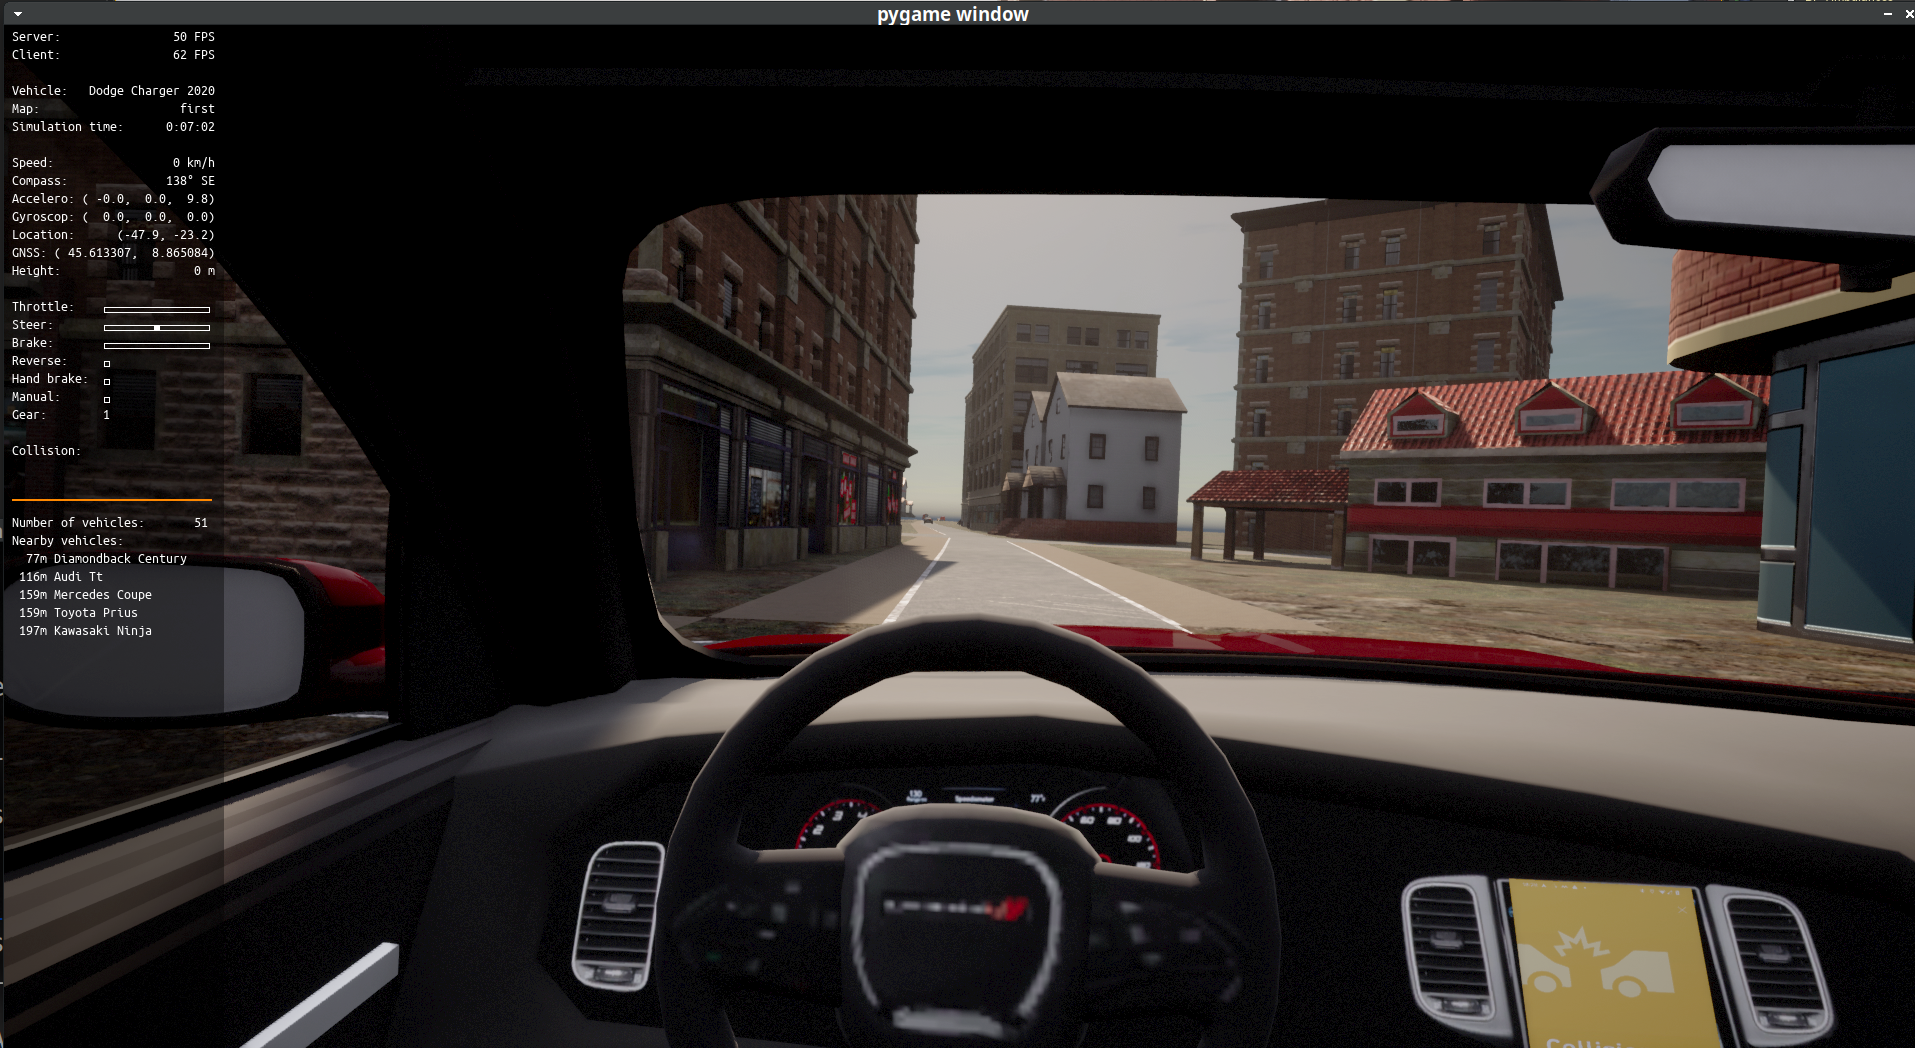
\includegraphics[height=\textheight, keepaspectratio, width=\linewidth]{CARLAScreenshot.png}
\column{0.48\linewidth}
    \begin{itemize}
        \item We want to calibrate car \textbf{\textcolor{red}{accident prediction}} algorithms
        \item Corporate will \textbf{not} let us use real humans 
        \item Simulations must be efficient because of machine learning.
        \item How do we maintain a \textbf{\textcolor{red}{ever increasing}} library of simulated scenarios?
    \end{itemize}
\end{columns}

\end{frame}



\begin{frame}[fragile]{Defining interactive components}
    A \textbf{\textcolor{red}{interactive component}} is a program component which behaviour depends on some input, and the input depends on the component behaviour.

    \centering
\makebox[\textwidth][c]{%
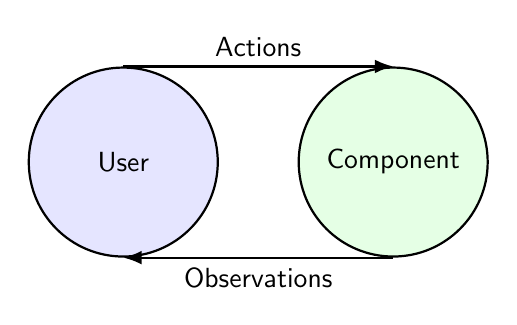
\begin{tikzpicture}[
  >=Latex,
  every node/.style={font=\sffamily},
  role/.style={circle,draw,thick,minimum size=2.4cm,align=center,inner sep=0pt},
  agent/.style={role,fill=blue!10},
  env/.style={role,fill=green!10}
]
  % Nodes
  \node[agent] (agent) {User};
  \node[env,right=of agent] (env) {Component};

  % Arrows
  \draw[->,thick, above, bend left=30] (agent.north) -- node[above]{Actions} (env.north);
  \draw[->,thick, below] (env.south) -- node[below]{Observations} (agent.south);

\end{tikzpicture}
}
\end{frame}

\begin{frame}[fragile]{Examples of interactive components}
    \begin{itemize}
        \item A website with a multipage form
        \item A chess simulation to train AI agents
        \item The TCP protocol 
        \item A load balancing algorithm that spawns and tears down servers depending on the state of the network
    \end{itemize}
\end{frame}

\begin{frame}[fragile]{Often but not always}
    \begin{itemize}
        \item Often \textbf{\textcolor{red}{interactive components}} are part of larger systems
        \item Often \textbf{\textcolor{red}{interactive components}} are a small part of a programmer's job
    \end{itemize}
        Techniques to design, implement and maintain interactive components are not commonly known
    \linebreak
    \begin{itemize}
        \item Often \textbf{\textcolor{red}{interactive components}} are mandated by business requirements and/or third party specification documents
        \item Often  \textbf{\textcolor{red}{interactive components}} start simple and then grow in complexity as features are added. 
    \end{itemize}
       Changes in requirements sometimes push, without programmers noticing, the system in a entirely new category of complexity that forces to rewrite the whole component.
\end{frame}


%\begin{frame}{Lack of cathegories to talk about interactive programs}
   %\noindent 
   %\center
    %\includegraphics[height=0.6\textheight, keepaspectratio, width=\linewidth]{1520215053505.jpeg}

    %Precise words to talk about datastructures properties \newline Imprecise words to talk about interactive components properties


%\end{frame}

\begin{frame}[fragile]{Running example}

The user rolls to dices and sums them. If the result is less than 7 the user is allowed to reroll. Otherwise the user can add a number between 0 and 5 to the result. 

\begin{lstlisting}[style=cppstyle]
void runningExample() {
    int result = rollTwoDice();
    if (result < 7 && userWantsToReroll()) {
        result = rollTwoDice();
        return;
    }

    result += userDecidedQuantity();
}
\end{lstlisting}


\textbf{userWantsToReroll} and \textbf{userDecidedQuantity} are user actions.

\textbf{rollTwoDice} is a random event, independent from user actions. 
\end{frame}


\section{Interactive components original sin: \\ \noindent \textcolor{red}{thread blocking}}
\begin{frame}[fragile]{No main loop}
    Functions either block the current thread or they do not. 

\begin{lstlisting}[style=cppstyle]
void runningExample() {
    int result = rollTwoDice();
    if (result < 7 && userWantsToReroll()) { // waits for user input
        result = rollTwoDice();
        return;
    }

    result += userDecidedQuantity(); // waits for user input
}
\end{lstlisting}
    Blocking is often unacceptable. Spawning a thread is sometimes too costly.
\end{frame}

\begin{frame}[fragile]{Examples:}

\begin{lstlisting}[style=cppstyle]
void graphical_engine_main_loop(Engine& engine) {  // interactive
    while (not engine.is_done()){
        engine.render_and_display_frame(); // not interactive
        engine.query_inputs();             // not interactive
        engine.simulation_step();          // interactive
    }}
\end{lstlisting}

\begin{lstlisting}[style=cppstyle]
void machine_learning_chess_engine(NeuralNetwork& nn, Game& game) {  
    while (not game.is_done()){
        Move move = nn.select_action(game.observe());  // not interactive
        game.apply_move(move);                         // interactive 
    }}
\end{lstlisting}
The engine owns the main loop, the application logic cannot have it.
\end{frame}

\begin{frame}[fragile, plain]{Class rewriting}
  \begin{columns}[T,onlytextwidth]
\begin{column}{0.50\textwidth}
\begin{lstlisting}[style=cppstyle,numbers=none]
void runningExample() {


  int result = rollTwoDice();
  if (result < 7 && 
        userWantsToReroll()) { 


    result = rollTwoDice();
    return;
  }

  result += userDecidedQuantity(); 
}
\end{lstlisting}
\end{column}
    \begin{column}{0.48\textwidth}
\begin{lstlisting}[style=cppstyle,numbers=none]
struct RunningExample {
 int next = 0; int result;
 void start() { assert(next == 0);
  result = rollTwoDice();
  next = result < 7 ? 1 : 2;
 }
 void userRerolls(bool it_does) { 
  assert(next == 1);
  if (it_does)
    result = rollTwoDice();
  next = it_does ? -1 : 2;
 }
 void userDecidesQuantity(int q) { 
  assert(next == 2);
  result += q;
  next = -1;
 }
\end{lstlisting}
\end{column}
\end{columns}

\end{frame}


%\begin{frame}[fragile]{Let us look at the assembly}

  %\begin{columns}[T,onlytextwidth]
%\begin{column}{0.50\textwidth}
%\begin{lstlisting}[style=cppstyle,numbers=none]
%void runningExample() {
  %int result = rollTwoDice();

  %if (result < 7 && 

        %userWantsToReroll()) { 



    %result = rollTwoDice();
    %return;}
  %result += userDecidedQuantity(); 
%}
%\end{lstlisting}
%\end{column}
    %\begin{column}{0.48\textwidth}
%\begin{lstlisting}[style=cppstyle,numbers=none]
      %push    rbx
      %call    rollTwoDice()
      %mov     ebx, eax
      %cmp     eax, 6
      %jg      .L2
      %call    userWantsToReroll()
      %test    al, al
      %jne     .L2
      %pop     rbx
      %jmp     rollTwoDice()
      %ret
%.L2:  call    userDecidedQuantity()
      %add     eax, ebx
      %pop     rbx
      %ret
%\end{lstlisting}
%\end{column}
%\end{columns}
%\end{frame}

%\begin{frame}[fragile, plain]

  %\begin{columns}[T,onlytextwidth]
%\begin{column}{0.50\textwidth}
%\begin{lstlisting}[style=cppstyle,numbers=none]
%struct RunningExample {
 %int next = 0; int result;
 %void start() { 
  %result = rollTwoDice();


  %next = result < 7 ? 1 : 2;}
 %void userRerolls(bool it_does) { 

  %if (it_does)

    %result = rollTwoDice();
  %next = -1;
 %}

 %void userDecidesQuantity(int q) { 
  %result += q;

  %next = -1;}
%\end{lstlisting}
%\end{column}
    %\begin{column}{0.48\textwidth}
%\begin{lstlisting}[style=cppstyle,numbers=none]
      %push    rbx


      %call    rollTwoDice()
      %mov     ebx, eax
      %cmp     eax, 6
      %jg      .L2
      %call    userWantsToReroll()
      %test    al, al
      %jne     .L2
      %pop     rbx
      %jmp     rollTwoDice()
      %ret


%.L2:  call    userDecidedQuantity()
      %add     eax, ebx
      %pop     rbx
      %ret
%\end{lstlisting}
%\end{column}
%\end{columns}
%\end{frame}

\begin{frame}[fragile]{Manual state managment $\equiv$ Unstructured control flow}

Exploiting a new variable to keep track of the point we are at in the program is equivalent to unstructured programming.
    \begin{table}[h]
\centering
\begin{tabular}{|l|l|l|}
\hline
\textbf{Class implementation} & \textbf{Unstructured C} & \textbf{Assembly} \\
\hline
\texttt{next} &  & \texttt{program counter} \\
\texttt{next = 2} & \texttt{goto label2} & \texttt{jmp label2} \\
\texttt{next = cond ? 1 : 2} & \texttt{switch (cond) \{...\}} & \texttt{cbr cond label1 label2} \\
\texttt{next = -1} & \texttt{return} & \texttt{ret} \\
\hline
\end{tabular}


\end{table}


\end{frame}
\begin{frame}[fragile]{Class rewrites are inherently complex to manage}
    \centering
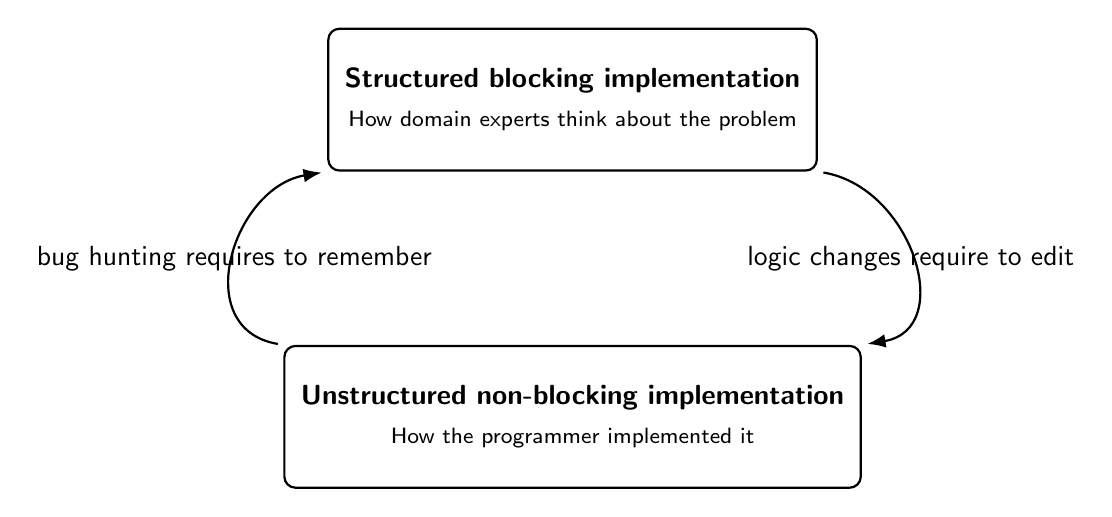
\begin{tikzpicture}[
  node distance=2.2cm,
  >=Latex,
  every node/.style={align=center},
  box/.style={draw, rounded corners, thick, minimum width=6.2cm, minimum height=1.8cm, inner sep=6pt}
]
% Nodes (stacked)
\node[box] (structured) {\textbf{Structured blocking implementation}\\[2pt]
\footnotesize How domain experts think about the problem};

\node[box, below=of structured] (unstructured) {\textbf{Unstructured non-blocking implementation}\\[2pt]
\footnotesize How the programmer implemented it};

% Curved arrows, routed on opposite sides to avoid overlap
\draw[->, thick, shorten >=2pt, shorten <=2pt]
  (structured.south east)
    .. controls +(1.2,-0.2) and +(1.2,0.2) ..
  node[pos=0.5] {logic changes require to edit}
  (unstructured.north east);

\draw[->, thick, shorten >=2pt, shorten <=2pt]
  (unstructured.north west)
    .. controls +(-1.2,0.2) and +(-1.2,-0.2) ..
  node[pos=0.5] {bug hunting requires to remember}
  (structured.south west);

\end{tikzpicture}


\end{frame}


\begin{frame}{Class rewriting, general methods}
  \begin{block}{Questions?}
      \begin{itemize}
          \item Can any blocking function be rewritten as a class?
              \linebreak \textcolor{blue}{yes}
          \item Is there a general algorithm to convert a function into a class? 
              \linebreak \textcolor{blue}{yes: Control flow flattening in compilers, state machine syntesys in hardware design}
          \item Can GCC, CLANG or MSVC do it for me? 
              \linebreak \textcolor{orange}{If coroutines are enough, yes}
    \end{itemize}
  \end{block}
\end{frame}

%\begin{frame}[fragile]{Flattening, concepts}
    %\begin{itemize}
        %\item Algorithm used in compilers and hardware design.
        %\item For each control flow statement (if, while, for...) that contains a blocking operation, starting from the most nested one:
            %\begin{itemize}
                %\item rewrite it using only gotos
            %\end{itemize}
    %\end{itemize}

  %\begin{columns}[T,onlytextwidth]
    %\begin{column}{0.50\textwidth}
%\begin{lstlisting}[style=cppstyle,numbers=none]
%if (condition) 
    %if (condition2) 
        %blocking();
%if (condition3) nonBlocking();
%\end{lstlisting}

%\end{column}
    %\begin{column}{0.48\textwidth}
%\begin{lstlisting}[style=cppstyle,numbers=none]
%switch (state) {
%case ID0:
 %state = condition?ID1:ID2;break;
%case ID1:
 %state = condition?ID3:ID2;break;
%case ID3
 %blocking(); 
 %state=ID2;break;
%case ID2
 %if (condition3) nonBlocking();}
%\end{lstlisting}
    %\end{column}
%\end{columns}
            
%\end{frame}

%\begin{frame}[fragile]{Flattening, concepts}
%\begin{lstlisting}[style=cppstyle,numbers=none]
%void execute() {
  %while (true) {
    %switch (state) {
      %case ID0:
       %state = condition && condition2 ? ID3 : ID2;
       %break;

      %case ID3
       %state = ID2;
       %break;
      %case ID2
       %if (condition3) 
         %nonBlocking();
    %}
  %}}
%\end{lstlisting}
%\end{frame}

\begin{frame}[fragile, plain]{Coroutines digression}

\noindent
  \begin{columns}[T,onlytextwidth]
    \begin{column}{0.50\textwidth}
\begin{lstlisting}[style=cppstyle,numbers=none]
Task runningExample(Input<bool>& reroll, Input<int>& quantity) {
  int result = rollTwoDice();
  if (result < 7) {
    bool do_reroll = co_await reroll;
    if (do_reroll) {
      result = rollTwoDice();
      co_return result;               
    }
  }
  result += co_await quantity;
  co_return result;}
\end{lstlisting}
\end{column}
    \begin{column}{0.45\textwidth}
\begin{lstlisting}[style=cppstyle,numbers=none]
int main() {
  Input<bool> reroll;
  Input<int>  quantity;
  Task t = runningExample(reroll, quantity);
  t.start(); 
  reroll.supply(false); 
  quantity.supply(3);
  if (t.done()) {
    print("done") 
  }
}
\end{lstlisting}
    \end{column}
\end{columns}

CPP coroutines are not copiable or serializable. Copiable/serializable strongly typechecked zero-overhead coroutines are very challenging to implement. 

\end{frame}

\begin{frame}{Original sin, conclusion}
\begin{itemize}
    \item Some use cases require the main loop. (web servers, graphical engines...)
    \item The interactive component cannot have it too.

\end{itemize}
    \begin{block}{Solutions:}
\begin{itemize}
    \item Spawn a thread. \textbf{\textcolor{red}{costly}} \textbf{\textcolor{blue} {simple}}
    \item Coroutines. \textbf{\textcolor{blue}{one malloc / free per coroutine creation, but manually optimizable}} \textbf{\textcolor{orange}{complex at the start, easy afterward}} \textcolor{red}{\textbf{not copiable/serializable}}
    \item Rewrite as a class. \textbf{\textcolor{blue}{1 extra integer cost in most situations}} \textbf{\textcolor{red}{Easy at the start, complex to maintain}}
\end{itemize}
    \end{block}
\end{frame}

\begin{frame}{Acceptable implementations}
\renewcommand{\arraystretch}{1.3} % more vertical padding
\setlength{\tabcolsep}{3pt}       % horizontal padding


\begin{tabularx}{\textwidth}{l|c|c|c|c}
\hline
 & \textbf{No calls}
 & \textbf{Non Recursive}
 & \textbf{Recursive}
 & \textbf{Turing complete} \\
\hline
    \textbf{Non serializable}       &  \multicolumn{3}{|c|}{threads - coroutines }   \\
\hline
\textbf{Serializable}        &  &  &  &   \\
\hline
\end{tabularx}
\end{frame}

\begin{frame}{Systems grow in complexity}
    \begin{itemize}
        \item Domain experts often promise to never copy the state of interactive components, and then want to copy it. (Example: "In the car simulator, I want to copy the behaviour of a car, modify it, and after a while restore it to the previous behaviour")
        \item Often you want to isolate user actions in their own functions. 
    \end{itemize}

    \textbf{\textcolor{red}{If your solution cannot handle serialization and/or calls, you will have to rewrite the system.}}

    %When the user actions become complex, writing the class becomes extreamly taxing.
    %\centering
  %\includegraphics[height=0.8\textheight, keepaspectratio, width=0.8\linewidth]{afg.png}
\end{frame}

\begin{frame}{Turing complete?}
Interactive systems where a user can provide an arbitrary program as input:
\begin{itemize}
    \item The python interpreter
    \item A moddable videogame 
\end{itemize}

\textbf{\textcolor{red} {Solution:}} interpreter / just in time compiler
\renewcommand{\arraystretch}{1.3} % more vertical padding
\setlength{\tabcolsep}{3pt}       % horizontal padding


\begin{tabularx}{\textwidth}{l|c|c|c|c}
\hline
 & \textbf{No calls}
 & \textbf{Non Recursive}
 & \textbf{Recursive}
 & \textbf{Turing complete} \\
\hline
    \textbf{Non serializable}       &  \multicolumn{3}{|c|}{threads - coroutines } & interpreter  - jit \\
\hline
\textbf{Serializable}        &  &  &  &  interpreter - jit\\
\hline
\end{tabularx}
\end{frame}

\begin{frame}{Serializable interactive components that scales}
    We need a way to implement those systems:
    \begin{itemize}
        \item Minimizing the distance between the mental model of the domain experts and of the implementation 
        \item With as little overhead as possible
        \item With theoretical guarantees that expanding the implementation will not break the design.
    \end{itemize}
    
    State machines with extra tricks meet our requirements. 
\end{frame}

%\begin{frame}[fragile]{What do other people do? Unreal engine blueprints}
    %\centering
    %\includegraphics[height=0.8\textheight, keepaspectratio, width=0.8\linewidth]{bpqs_5_step8.png}

    %Graphical scripting languages minimize the distance between mental model and concrete code, with fairly low performance degradation.
%\end{frame}
\begin{frame}[fragile, plain]{Serializable, no-calls interactive component}

    No calls interactive components are interactive components where all user actions appear in a single function. 

    

    \centering
\makebox[\textwidth][c]{%
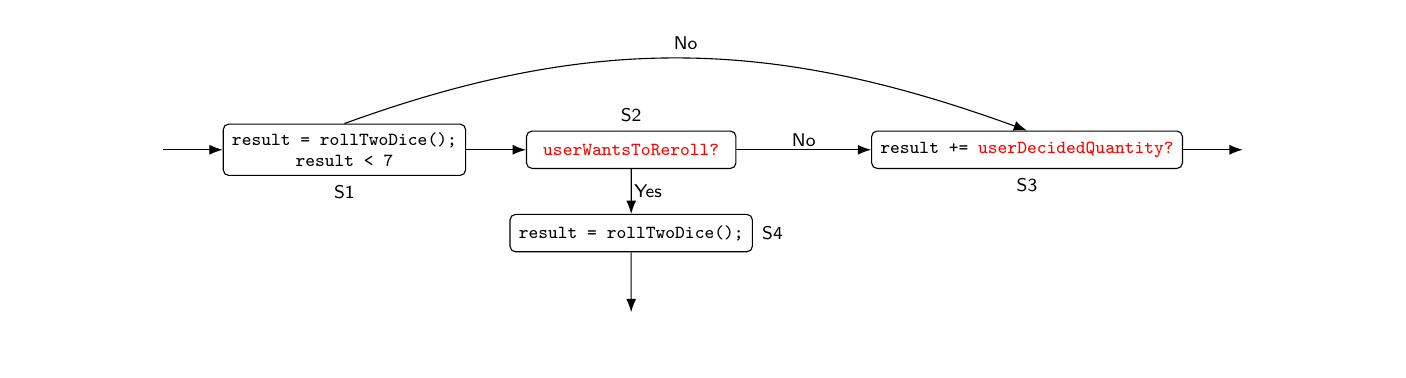
\begin{tikzpicture}[
  >=Latex,
  node distance=8mm and 8mm,
  every node/.style={font=\scriptsize},
  startstop/.style={minimum width=18mm, minimum height=5mm, align=center},
  process/.style={rectangle, draw, rounded corners=2pt, minimum width=28mm, minimum height=5mm, align=center},
  decision/.style={diamond, draw, aspect=1.7, inner ysep=0.6ex, align=center},
  arrow/.style={-Latex, thin},
  scale=0.95, transform shape
]

% Row (left -> right)
\node[startstop] (start) {};
\node[process, right=of start, label=below:{\scriptsize S1}] (init) {\texttt{result = rollTwoDice();} \\ \texttt{result < 7}};
\node[process, right=of init, , label=above:{\scriptsize S2}] (condB) {\texttt{\textcolor{red}{userWantsToReroll?}}};
\node[process, right=18mm of condB, label=below:{\scriptsize S3}] (accum) {\texttt{result += \textcolor{red}{userDecidedQuantity?}}};
\node[startstop, right=of accum] (end) {};

% Small downward branch for the reroll+return
\node[process, below=6mm of condB, , label=right:{\scriptsize S4}] (reroll) {\texttt{result = rollTwoDice();}};
\node[startstop, below=of reroll] (ret) {};

% Edges (left to right primary flow)
\draw[arrow] (start) -- (init);
\draw[arrow] (init) -- (condB);

% Split && into two nodes

% condA No -> accum (skip second test)
\draw[arrow] (init.north) to[out=20,in=160] node[above,pos=0.5]{No} (accum.north);

% condB Yes -> reroll -> return
\draw[arrow] (condB) -- node[right, inner sep=1pt]{Yes} (reroll);
\draw[arrow] (reroll) -- (ret);

% condB No -> accum
\draw[arrow] (condB) -- node[above, inner sep=1pt]{No} (accum);

% accum -> end
\draw[arrow] (accum) -- (end);


\end{tikzpicture}

}

\flushleft{
Common, but often you want to isolate sections into subfunctions to reuse them, even when you could just write everything in a single one.}

\end{frame} 

\begin{frame}[fragile, plain]{A possible implementation of a state machine library}

  \begin{columns}[T,onlytextwidth]
\begin{column}{0.50\textwidth}
\begin{lstlisting}[style=cppstyle, numbers=none]
STATE_MACHINE(resume) {

    STATE(S1)
    NEXT(S2)
    ....
    DECISION(S2):
    ...
}
\end{lstlisting}

\end{column}
\begin{column}{0.48\textwidth}
\begin{lstlisting}[style=cppstyle, numbers=none]
void resume(Args args) {
    switch(state) {
labelS1: case S1: // S1 == 0
    goto labelS2;
    ....
labelS2: state=S2; return; case S2:
    ...
    }
}
\end{lstlisting}
\end{column}
\end{columns}
\textbf{labelS2: state=S2;} allows us remember where we are.

\textbf{return;} stops the execution. 

\textbf{case S2:} resumes the execution from the current line.
\end{frame}



\begin{frame}[fragile, plain]{Conversion to CPP}

  \begin{columns}[T,onlytextwidth]
\begin{column}{0.52\textwidth}
\begin{lstlisting}[style=cppstyle, numbers=none]
class RunningExample {
  STATE_MACHINE(resume, {
    STATE(S1):
      result = rollTwoDice();
    NEXT(result < 7, S2, S4)
    DECISION(S2):
    NEXT(userWantsToReroll, S3, S4)
    STATE(S3):
      result = rollTwoDice();
    NEXT(END)
    DECISION(S4):
      result += userDecidedQuantity;
    NEXT(END)
    });
\end{lstlisting}

\end{column}
\begin{column}{0.45\textwidth}
\begin{lstlisting}[style=cppstyle, numbers=none]
  enum State {
    S1,S2,S3,S4,END
  };
  int result; States state; 
  void start() {
    assert(state == S1);
    resume();
  }
  ACT(S2, do_reroll, 
      bool, userWantsToReroll)

  ACT(S4, decide_quantity, 
      int, userDecidedQuantity)
};
\end{lstlisting}
\end{column}
\end{columns}
\end{frame}

\begin{frame}[fragile, plain]

  \begin{columns}[T,onlytextwidth]
\begin{column}{0.50\textwidth}
\begin{lstlisting}[style=cppstyle, numbers=none]
void resume() {
 switch (state) {
  case S1:
   result = rollTwoDice();
   if (result < 7)
    goto labelS2;
   else
    goto labelS3
labelS2: state=S2; return; case S2:
   if (userWantsToReroll)
    goto labelS4;
   else
    goto labelS3;
labelS3: 
   result = rollTwoDice();  
   goto labelEND;
labelS4: state=S4; return; case S4:
   result += userDecidedQuantity;
   goto labelEND;
labelEND: state = END; case END:
        return;
    }}
\end{lstlisting}

\end{column}
\begin{column}{0.45\textwidth}
\begin{lstlisting}[style=cppstyle, numbers=none]
  enum State {S1, S2, S3, END};
  int result; States state; 
  void start() {
    assert(state == S1);
    resume();
  }
  bool userWantsToReroll;
  void do_reroll(bool userWantsToReroll) {
    assert(state == S2);
    this->userWantsToReroll = userWantsToReroll;
    resume();
  }
  int userDecidedQuantity;
  void decide_quantity(int userDecidedQuantity) {
    assert(state == S4);
    this->userDecidedQuantity = userDecidedQuantity;
    resume();
  }
  };
\end{lstlisting}
\end{column}
\end{columns}
\end{frame}


\begin{frame}{Acceptable implementations}
\renewcommand{\arraystretch}{1.3} % more vertical padding
\setlength{\tabcolsep}{3pt}       % horizontal padding


\begin{tabularx}{\textwidth}{l|c|c|c|c}
\hline
 & \textbf{No calls}
 & \textbf{Non Recursive}
 & \textbf{Recursive}
 & \textbf{Turing complete} \\
\hline
    \textbf{Non serializable}       &  \multicolumn{3}{|c|}{threads - coroutines - rewrites} & interpreter  \\
\hline
\textbf{Serializable}        & STM &  &  &  interpreter \\
\hline
\end{tabularx}
\end{frame}

\begin{frame}[fragile, plain]{Non-recursive non-blocking interactive functions}
Actions may be located in multiple functions, but no functions is ever active more than once. Isolation of concerns makes this the most common scenario.
\makebox[\textwidth][c]{%
    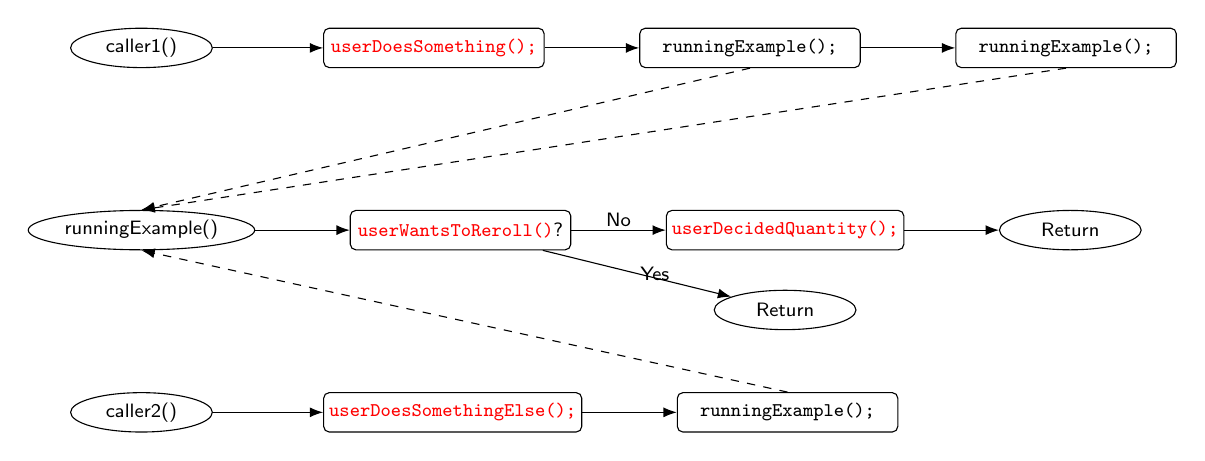
\begin{tikzpicture}[
  >=Latex,
  node distance=7mm and 12mm,
  every node/.style={font=\scriptsize},
  % Styles
  func/.style={rectangle, draw, rounded corners=2pt, align=center, inner sep=2pt, minimum width=22mm},
  startstop/.style={ellipse, draw, align=center, inner sep=1.2pt, minimum width=18mm, minimum height=5mm},
  process/.style={rectangle, draw, rounded corners=2pt, align=center, inner sep=2pt, minimum width=28mm, minimum height=5mm},
  decision/.style={diamond, draw, aspect=1.8, inner ysep=0.6ex, align=center},
  flow/.style={-Latex, thin},          % control-flow (solid)
  call/.style={-Latex, dashed, thin},  % call-graph (dashed)
  lbl/.style={font=\scriptsize, inner sep=1pt}
]

% =======================
% Function titles (vertical column)
% =======================
\node[startstop] (f1) {caller1()};
\node[startstop, below=18mm of f1] (re_entry) {runningExample()};
\node[startstop, below=18mm of re_entry] (f2) {caller2()};

% =======================
% caller1 content (left -> right)
% =======================
\node[process, right=14mm of f1] (c1a) {\texttt{\textcolor{red}{userDoesSomething();}}};
\node[process, right=of c1a] (c1b) {\texttt{runningExample();}} % first call site
;
\node[process, right=of c1b] (c1c) {\texttt{runningExample();}} % second call site
;

\draw[flow] (f1.east) -- (c1a.west);
\draw[flow] (c1a) -- (c1b);
\draw[flow] (c1b) -- (c1c);

% =======================
% runningExample content (left -> right)
% =======================
\node[process, right=of re_entry] (re_cond) {\texttt{\textcolor{red}{userWantsToReroll()}}?};
\node[process, right=of re_cond] (re_do) {\texttt{\textcolor{red}{userDecidedQuantity();}}};
\node[startstop, below=5mm of re_do] (re_ret) {Return};
\node[startstop, right=of re_do] (re_end) {Return};

\draw[flow] (re_entry) -- (re_cond);
\draw[flow] (re_cond) -- node[right, lbl]{Yes} (re_ret);
\draw[flow] (re_cond) -- node[above, lbl]{No} (re_do);
\draw[flow] (re_do) -- (re_end);

% =======================
% caller2 content (left -> right)
% =======================
\node[process, right=14mm of f2] (c2a) {\texttt{\textcolor{red}{userDoesSomethingElse();}}};
\node[process, right=of c2a] (c2b) {\texttt{runningExample();}} % call site
;

\draw[flow] (f2.east) -- (c2a.west);
\draw[flow] (c2a) -- (c2b);

% =======================
% Call graph edges (dashed) to runningExample ONLY
% (added after layout; they don't affect node positions)
% =======================
\draw[call] (c1b.south) to (re_entry.north);
\draw[call] (c1c.south) to (re_entry.north);
\draw[call] (c2b.north) to (re_entry.south);

\end{tikzpicture}
}
\end{frame}

\begin{frame}[fragile, plain]{Solution, introduce CALL/RETURN macros}
\begin{columns}[T,onlytextwidth]
\begin{column}{0.50\textwidth}
\begin{lstlisting}[style=cppstyle, numbers=none]
CALL(runningExample, C1)
\end{lstlisting}
\end{column}
\begin{column}{0.48\textwidth}
\begin{lstlisting}[style=cppstyle, numbers=none]
ret_addresses.push_back(C1);
goto runningExample;
case C1:
\end{lstlisting}
\end{column}
\end{columns}

\begin{columns}[T,onlytextwidth]
\begin{column}{0.50\textwidth}
\begin{lstlisting}[style=cppstyle, numbers=none]
RETURN()
\end{lstlisting}
\end{column}
\begin{column}{0.48\textwidth}
\begin{lstlisting}[style=cppstyle, numbers=none]
while (true) {
  switch(state) {
    ...
    state = ret_addresses.back()
    ret_addresses.pop_back();
    continue;
    ...
  }
}
\end{lstlisting}
\end{column}
\end{columns}
Extra memory footprint < 1 integer per function + 1.
\end{frame}



\begin{frame}{Acceptable implementations}
\renewcommand{\arraystretch}{1.3} % more vertical padding
\setlength{\tabcolsep}{3pt}       % horizontal padding


\begin{tabularx}{\textwidth}{l|c|c|c|c}
\hline
 & \textbf{No calls}
 & \textbf{Non Recursive}
 & \textbf{Recursive}
 & \textbf{Turing complete} \\
\hline
    \textbf{Non serializable}       &  \multicolumn{3}{|c|}{threads - coroutines} & interpreter  \\
\hline
\textbf{Serializable}        & STM & STM+CALL/RET &  &  interpreter \\
\hline
\end{tabularx}
\end{frame}

\begin{frame}[fragile, plain]{Recursive interactive systems}
User actions are located in functions that can call directly or indirectly themselves.
Rare: code editor command stacks, videogames.
\begin{columns}[T,onlytextwidth]
\begin{column}{0.50\textwidth}
\begin{lstlisting}[style=cppstyle, numbers=none]
CALL(runningExample, C1)
\end{lstlisting}
\end{column}
\begin{column}{0.48\textwidth}
\begin{lstlisting}[style=cppstyle, numbers=none]
stack_frames.emplace_back(RunningExample());
stack_frames.back().start();
state = C1;
return;
\end{lstlisting}
\end{column}
\end{columns}


Requires dynamic memory (unless recursion is bounded), cost is proportional to the longest recursion chain.
\end{frame}


\begin{frame}[fragile, plain]

    \begin{tikzpicture}[node distance=20mm and 25mm, every node/.style={align=center}]

% Q1
\node[decision] (q1) {Is your interactive\\component Turing-complete?};

% Yes -> Interpreter/JIT
\node[block, right=20mm of q1] (jit) {Interpreter / JIT};
\draw[line] (q1) -- node[lbl,above]{Yes} (jit);

% No -> Q2
\node[decision, below=9mm of q1] (q2) {Any reason now or in the future to\\copy/serialize state \emph{or}\\do you need the best performance?};
\draw[line] (q1) -- node[lbl,left]{No} (q2);

% Q2 No -> Coroutines/Threads
\node[block, below left=16mm and 2mm of q2] (coro) {Coroutines / Threads};
\draw[line] (q2.west) -- ++(-10mm,0) |- node[pos=0.30, lbl,left]{No} (coro.north);

% Q2 Yes -> Q3
\node[decision, below right=4mm and 6mm of q2] (q3) {Does it recursively call\\functions with user\\actions inside?};
\draw[line] (q2.east) -- ++(10mm,0) |- node[pos=0.3, lbl,right]{Yes} (q3.north);

% Q3 No -> State machine + non-recursive
\node[block, below left=8mm and 6mm of q3] (smnonrec) {State machine\\+ non-recursive calls};
\draw[line] (q3.west) -- ++(-10mm,0) |- node[pos=0.3, lbl,left]{No} (smnonrec.north);

% Q3 Yes -> State machine + recursive
\node[block, below=8mm of q3] (smrec) {State machine\\+ recursive calls};
\draw[line] (q3.south) -- ++(00mm,0) |- node[pos=0.3, lbl,right]{Yes} (smrec.north);

\end{tikzpicture}
%\renewcommand{\arraystretch}{1.3} % more vertical padding
%\setlength{\tabcolsep}{3pt}       % horizontal padding
%\begin{tabularx}{\textwidth}{l|c|c|c|c}
%\hline
 %& \textbf{No calls}
 %& \textbf{Non Recursive}
 %& \textbf{Recursive}
 %& \textbf{Turing complete} \\
%\hline
    %\textbf{Non serializable}       &  \multicolumn{3}{|c|}{threads - coroutines - class rewrites} & interpreter  \\
%\hline
%\textbf{Serializable}        & STM & STM+CALL/RET & CALL STACK  &  interpreter \\
%\hline
%\end{tabularx}
\end{frame}

\begin{frame}{Conclusions}
    \begin{itemize}
        \item Non blocking interactive systems force you into unstructured control flow
        \item The compiler knows what to do, but will not do it when you need serializable/copiable objects.
        \item State machines of various complexity are the best tool you have to keep track of the complexity, while having guaranteed bounds on their cost.
    \end{itemize}
\end{frame}



\begin{frame}{Thanks!}
  Massimo Fioravanti massimo.fioravanti@polimi.it \\
  Slides: \href{https://example.com}{example.com} \\
  Repo: \href{https://github.com/yourname/yourtalk}{github.com/yourname/yourtalk}
\end{frame}

\end{document}

